\chapter{Durchführung}
\label{cha:Durchführung}
In diesem Versuch wird ein Reflexklystron als Mikrowellensender verwendet, dessen funktionsweise in \autoref{cha:Theorie} genauer beschrieben ist. 
Als Stromzufuhr dient hier ein Netzteil. Diese erschaffenen Mikrowellen passieren zunächst einen Einweggleichrichter, welcher in entgegengesetzte Richtung
die Wellen stark dämpft.\\
Als nächstes Bauteil wird ein Frequenzmesser im MHz-Bereich verwendet und anschließend ein Abschwächer, welcher die Mikrowellenleistung in Abhängigkeit der Tiefe
einer Mikrometerschraube dämpfen kann. Dieser Grundaufbau ist für alle Teilversuche identisch.\\
An das offene Ende des Hohlleiters lassen sich nun entweder Abschluss oder Kurzschluss anschließen, wobei der Abschluss die Wellen absorbiert und der Kurzschluss diese
reflektiert. Als drittes mögliches Element kann eine Störstelle mit Abschluss verbaut werden, in welche sich eine Mikrometerschraube drehen lässt. Das Signal wird schließlich
mittels eines Detektors aufgenommen und auf einem SWR-Meter oder Oszilloskop wiedergegeben.\\
Der Grundaufbau des Versuchs ist bei jeden Versuchsteil gleich und ist in \autoref{fig:aufbau} gezeigt.
\begin{figure}
    \centering
    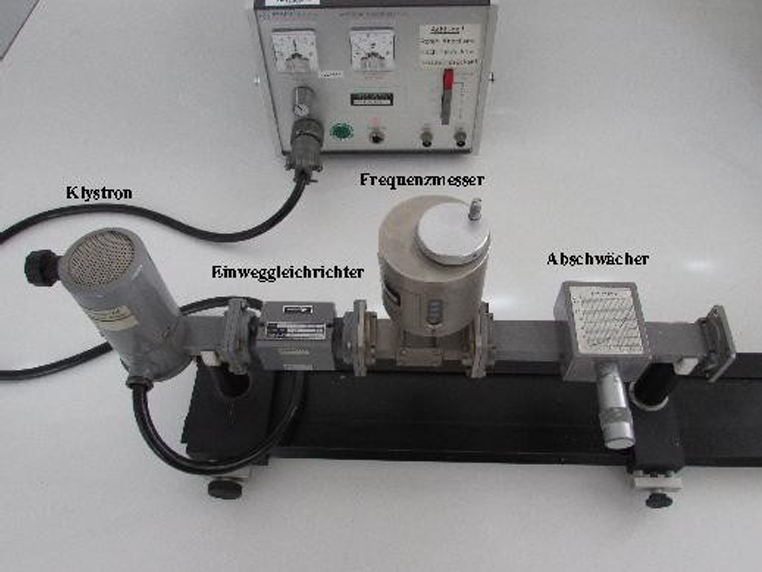
\includegraphics[scale=0.4]{content/V53_pictures/Aufbau.png}
    \caption{Verwendeten Grundaufbau für alle Versuchsteile. \cite{v53}}
    \label{fig:aufbau}
\end{figure}
\section{Kalibrierung des Versuchsaufbaus}
Das Klystron wird vor dem ersten Teilversuch etwa eine Minute vorgeheizt bei abgeschalteten \textit{Taster Res./Ref.}-Knopf. Um das Klystron zu kalibrieren wird der in \autoref{fig:Aufbau1} gezeigte
Aufbau verwendet.\\
Der Abschwächer wird auf $\qty{40}{\decibel}$ eingestellt, der $\qty{30}{decibel}$-Knopf des SWR-Meters gedrückt und der $\qty{1}{\kilo\hertz}$- und Verstärkungsdrehknauf in die mittlere Ausrichtung
gebracht. Am Klystron-Netzteil wird der $\qty{1}{\kilo\hertz}$-Modus verwendet und die Reflektorspannung auf etwa $\qty{100}{\volt}$ gestellt. Der  \textit{Taster Res./Ref.}-Knopf wird nun angeschaltet.\\
Die Reflektorspannung wird bei etwa $\qty{200}{\volt}$ so eingestellt, dass das SWR-Meter einen maximalen Ausschlag hat. Der Frequenzmesser wird anschließend so abgestimmt, dass sich ein Rückgang am SWR-Meter beobachten lässt.
\begin{figure}
    \centering
    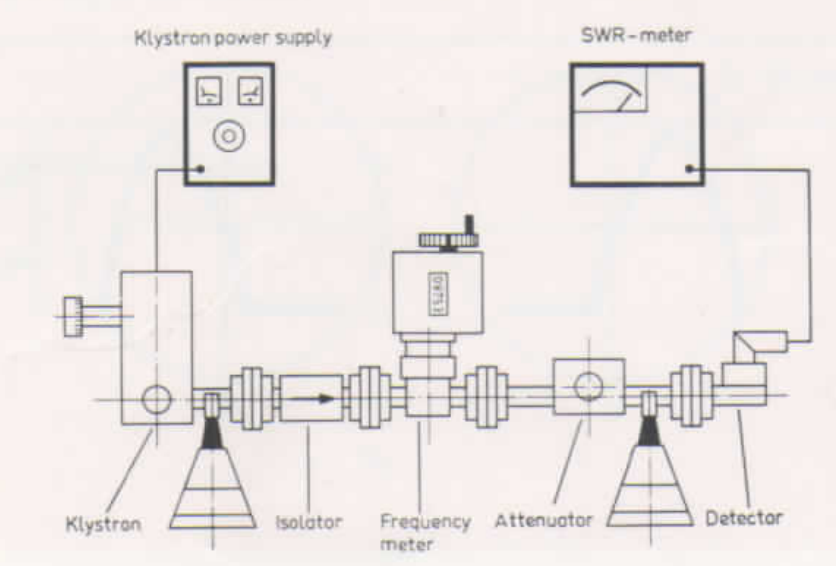
\includegraphics[scale=0.4]{content/V53_pictures/Aufbau1.png}
    \caption{Experimenteller Aufbau zur Kalibrierung des Klystrons. \cite{exp_mikro}}
    \label{fig:Aufbau1}
\end{figure}

\section{Untersuchung der Moden mittels Oszilloskop}
Für den ersten Teilversuch wird der Aufbau \autoref{fig:Aufbau2} verwendet. Hier wird lediglich SWR-Meter und Oszilloskop ausgetauscht.\\
Der Abschwächer wird auf $\qty{30}{\decibel}$ eingestellt und der Detektor mit dem Oszilloskop verbunden. Der andere Eingang des Oszilloskops wird mit dem \textit{0-30 V, 50 Hz} Ausgang des Netzteils verbunden und der Knopf 
\textit{50 Hz} auf dem Netzteil gedrückt. Bei ausgeschalteten \textit{Taster Res./Ref.}-Knopf lässt sich eine horizontale Linie auf dem Oszilloskop beobachten, welche mittig ausgerichtet werden soll.\\
Der \textit{Taster Res./Ref.}-Knopf wird anschließend wieder aktiviert und die Reflektorspannung auf etwa $\qty{200}{\volt}$ eingestellt. Die Reflektorspannung wird langsam verändert, bis sich eine deutliche Mode erkennen lässt.\\
Der Frequenzmesser wird wieder so eingestellt, bis sich eine Einkerbung (\textit{dip}) mittig in der Mode zeigt. So kann ermittelt werden, in welchen Frequenzbändern sich die Moden bewegen. Hierzu werden bei jeweils drei verschiedenen
Moden die Frequenzen, die Reflektorspannungen und relativen Amplitudenverhältnisse notiert, wo sich ein \textit{dip} in der Mitte und auf halber Höhe links und rechts vom Maximum zeigt.
\begin{figure}
    \centering
    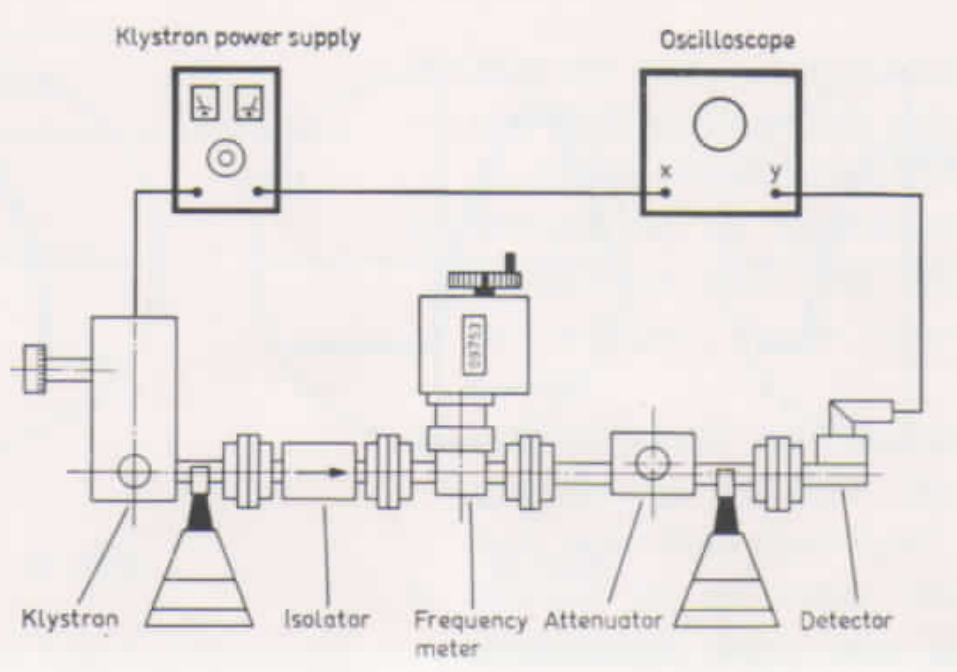
\includegraphics[scale=0.4]{content/V53_pictures/Aufbau2.png}
    \caption{Experimenteller Aufbau zur Untersuchung der Klystronmoden. \cite{exp_mikro}}
    \label{fig:Aufbau2}
\end{figure}

\section{Frequenz- und Wellenlängen-, und Dämpfungsmessung im Hohlleiter}
Im nächsten Teilversuch soll die Frequenz, Wellenlänge und Dämpfung unserer Welle im Hohlleiter bestimmt werden. Es wird der in \autoref{fig:aufbau3} gezeigte Aufbau verwendet.\\
Für alle drei Messungen wird zunächst der Abschwächer auf $\qty{20}{\decibel}$ eingestellt, der Detektor durch einen verschiebbaren Stehwellen-Detektor ersetzt und an das SWR-Meter angeschlossen. An den Detektor
wird zudem ein Abschluss angeschlossen.\\
Der $\qty{40}{\decibel}$-Knopf des SWR-Meters wird gedrückt, die Bandbreite auf  $\qty{100}{\hertz}$ gestellt und der $\qty{1}{\kilo\hertz}$- und Verstärkungsdrehknauf in die mittlere Ausrichtung
gebracht. Die Reflektorspannung des Netzteils wird auf circa $\qty{200}{\volt}$ eingestellt und der $\qty{1}{\kilo\hertz}$-Modus verwendet. Die Reflektorspannung wird verändert bis das SWR-Meter einen 
maximalen Ausschlag anzeigt. Mit dem $\qty{1}{\kilo\hertz}$-Knopf wird dieser Ausschlag maximal gemacht und der Bandbreitenschalter wieder auf $\qty{20}{\hertz}$ verringert.
\begin{figure}
    \centering
    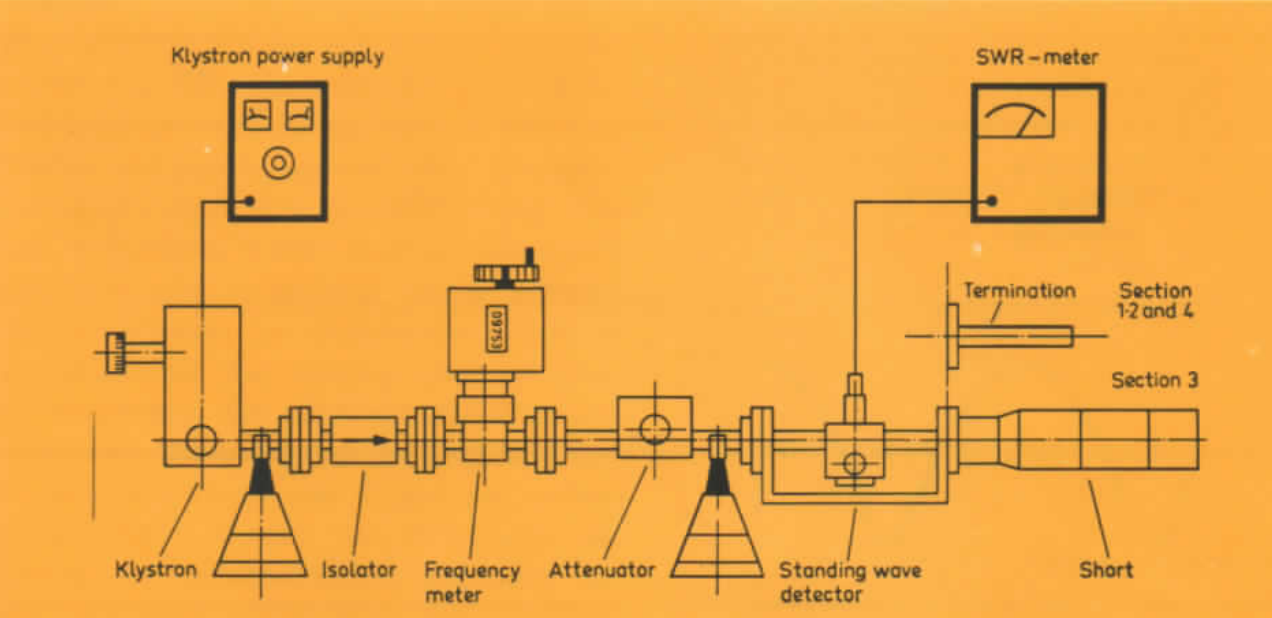
\includegraphics[scale=0.4]{content/V53_pictures/Aufbau3.png}
    \caption{Experimenteller Aufbau zur Untersuchung der Klystronmoden. \cite{exp_mikro}}
    \label{fig:aufbau3}
\end{figure}

\subsection{Frequenzmessung}
Um die Frequenz zu messen, wird der Frequenzmesser so lange gedreht, bis sich ein \textit{dip} am SWR-Meter zeigt. Diese Frequenz wird notiert.

\subsection{Wellenlängenmessung}
Für die Messung der Wellenlänge wird der Abschluss durch einen Kurzschluss ersetzt und der Frequenzmesser leicht verstimmt. Der Detektor wird entlang seiner Schiebe verschoben, bis der Ausschlag am SWR-Meter minimal ist.
Diese Stelle wird notiert. Anschließend wird der Detektor weitergeschoben bis zum nächsten \textit{dip}. Auch diese Stelle wird notiert.

\subsection{Messung der Dämpfung}
Für die Messung der Dämpfung des Abschwächers wird der Kurzschluss wieder durch einen Abschluss ersetzt. Das Klystron wird auf etwa $\qty{9}{\giga\hertz}$ abgestimmt und die Verstärkung am SWR Meter so eingestellt, dass 
ein Vollauschlag im $\qty{30}{\decibel}$-Bereich zu beobachten ist. Die Dämpfung wird durch drehen der Mikrometerschraube verstärkt und die Mikrometeranzeige in $\qty{2}{\decibel}$-Schritten auf der unteren Skala bis 
$\qty{10}{\decibel}$ notiert.

\section{Messung des Stehwellenverhältnisses}
Es wird ein ähnlicher Versuchsaufbau weiterverwendet. Der Kurzschluss wird durch eine Störstelle mit Abschluss ersetzt. Die Schraube an der Störstelle wird so weit reingedreht, bis eine Dämpfung sichtbar ist. Optimalerweise
sollte dies bei $\qty{0}{\micro\metre}$ der Fall sein. Der Abschwächer wird auf $\qty{20}{\decibel}$ eingestellt, der $\qty{40}{\decibel}$-Knopf
auf dem SWR-Meter gedrückt und der Bandbreitenschalter auf $\qty{20}{\hertz}$ gestellt. Die Einstellung des Klystrons können aus dem vorherigen Versuch übernommen werden. Im folgenden wird das Stehwellenverhältniss (SWR)
über drei verschiedene Methoden bestimmt.

\subsection{Direkte Methode}
Die Sondentiefe der Störstelle wird auf $\qty{5}{\milli\metre}$ erhöht. Der Detektor wird entlang seiner Schiene bis zu einem maximalen Ausschlag des SWR-Meters verschoben. Die Verstärkung des SWR-Meters wird so verstellt,
dass dieser maximale Ausschlag bei 1,0 auf der oberen Skala liegt. Die Sonde wird nun an eine Stelle minimalem Ausschlags verschoben. Der Wert auf der oberen Skala wird notiert. Die Stärke des Ausschlags wird für die Schraubentiefen
$0$ bis $\qty{10}{\milli\metre}$ gemessen.

\subsection{$\qty{3}{\decibel}$-Methode}
\label{subsec:3db_methode}

Die Sondentiefe der Störstelle wird auf $\qty{9}{\milli\metre}$ eingestellt. Der Detektor wird entlang seiner Schiene in ein Minimum gefahren. Die Verstärkung des SWR-Meters wird nun so eingestellt, dass auf der unteren Skala
$\qty{3}{\decibel}$ angezeigt werden. Die Sonde wird anschließend nach links verschoben bis sich ein Vollausschlag ergibt. Die jeweiligen Positionen des Detektors werden notiert. Der Detektor
wird nun nach rechts gefahren bis ein weiterer Vollauschlag auftritt. Auch diese Position wird notiert.

\subsection{Abschwächer-Methode}
\label{subsec:abschwächer}
Die Sondentiefe der Störstelle bleibt weiterhin auf $\qty{9}{\milli\metre}$. Der Detektor wird verschoben, bis sich ein Minimum am SWR-Meter zeigt. Die Verstärkung erneut so einstellen, dass sich ein Ausschlag von $\qty{3}{\decibel}$
ergibt. Der Detektor wird zeitgleich mit dem Abschwächer so verschoben/verstellt, dass der Ausschlag auf dem SWR-Meter ähnlich bleibt. Auf diese Weise wird ein relatives Maximum gesucht. Die entsprechende Abschwächung in der Endposition wird
notiert.